\documentclass[dvipsnames]{article}
\usepackage{pgfplots}
\usetikzlibrary{decorations.markings}
\pgfplotsset{compat=newest}

% \def\Point{36.9}

\begin{document}

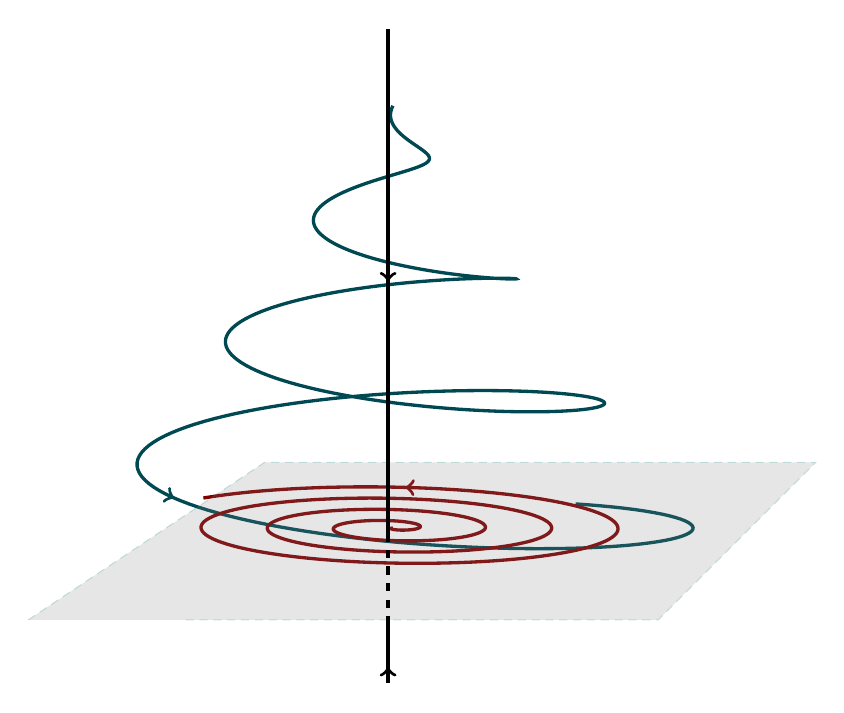
\begin{tikzpicture}
%левая
  \begin{axis}[
    view={-50}{-10}, %угол обзора
    axis lines=none,
    zmax=100,
    height=10cm,
    xtick=\empty,
    ytick=\empty,
    ztick=\empty
    ]
    \addplot3+[,ytick=\empty,yticklabel=\empty,
    mark=none,
    very thick,
    color={rgb,255:red,0; green,73; blue,83},
    domain=0:15*pi,
    postaction={decorate,
                decoration={markings,mark=at position 0.72 with {\arrow{>}}}
               },
    samples=400,
    samples y=0,
    ]
    ({x*sin(0.15*pi*deg(x))},{x*cos(0.15*pi*deg(x)},{-3.2*x+85});
    ]

    % \addplot3+[,ytick=\empty,yticklabel=\empty,
    % mark=none,
    % dashed, very thick,
    % color={rgb,255:red,0; green,73; blue,83},
    % domain=0:-5.5*pi,
    % postaction={decorate,
    %             decoration={markings,mark=at position 0.8 with {\arrow{<}}}
    %            },
    % samples=400,
    % samples y=0,
    % ]
    % (-{x*sin(-0.15*pi*deg(x))},{x*cos(0.15*pi*deg(x)},{x});
    % ]

    % \addplot3+[,ytick=\empty,yticklabel=\empty,
    % mark=none,
    % very thick,
    % color={rgb,255:red,0; green,73; blue,83},
    % domain=-5.5*pi:-15*pi,
    % postaction={decorate,
    %             decoration={markings,mark=at position 0.9 with {\arrow{<}}}
    %            },
    % samples=400,
    % samples y=0,
    % ]
    % (-{x*sin(-0.15*pi*deg(x))},{x*cos(0.15*pi*deg(x)},{x});

  \addplot3+[,ytick=\empty,yticklabel=\empty,
    mark=none,
    very thick,
    color={rgb,255:red,128; green,0; blue,0},
    domain=0:12*pi,
    postaction={decorate,
                decoration={markings,mark=at position 0.9 with {\arrow{>}}}
               },
    samples=400,
    samples y=0,
    ]
    ({x*sin(0.20*pi*deg(x))},{x*cos(0.20*pi*deg(x)},{-60});
    ]

  \end{axis}
  \draw[teal,densely dashed][fill = gray, opacity=0.2]  (0,0.5) -- (3,2.5) -- (10,2.5) -- (8,0.5) -- (2,0.5);
  \draw[very thick] [->] (4.57,5) --(4.57,4.8);
  \draw[very thick] (4.57,8) --(4.57,1.6);
  \draw[very thick, dashed] (4.57,1.6) --(4.57,0.3);
  \draw[very thick] (4.57,-0.3) --(4.57,0.45);
  \draw[very thick] [->] (4.57,-0.2) --(4.57,-0.1);

\end{tikzpicture}

\end{document}